% !TeX root = ../main.tex
% Add the above to each chapter to make compiling the PDF easier in some editors.

\section{Monoscopic Far-Field Rendering}
\subsection{Theory}
Monoscopic Far-Field Rendering (MFFR) is a curious approach strongly aligning with an inherent property of many optimizations in the field of rendering and real-time computing in general, which is the property of trading accuracy for speed. MFFR is a topic brought up again in the early days of Rift CV1's retail launch by [TODO: Oculus? Epic? check timeframe] at developer keynotes. \\
Understanding the concept requires some explanation of the technical and visual background. Proper depth perception of the human eye relies on the slight spatial distance between both eyes as each eye sees a slightly different angle of a given object. This difference in perceived angle is called stereo separation [TODO: word this more scientifically?] and without it, the brain has a hard to impossible time determining the depth of and at which a certain object or surface lies. Regular stereo rendering obviously recreates this separation correctly when rendering the two virtual eyes at their respective spatial offset from the HMD center - given correct projection and view matrices and accurate world scale at least. 
However, and that's one aspect MFFR exploits, as distance grows, stereo separation shrinks. In infinity, separation would be infinitely small, but even at more reasonable distances separation becomes so small that even with good vision it becomes hard to properly judge depth unless the object is large. This of course also holds true for rendered stereoscopy, but an additional limit is the pixel density of the output displays. What this means is that at a certain distance from the virtual camera, stereo separation will shrink to less than a full screen space pixel once projected. Obviously if the difference can physically not be displayed by the HMD, it seems a waste of resources to still render both eyes. \\
Mono Far-Field Rendering thus opts to skip the second view during rendering of the name-giving far field of objects. The hope here is that only rendering a single view past a certain distance reduces rendering load without the user noticing the theoretical loss in accuracy. 
This approach has caveats unfortunately. For one, the value at which a field split - the distance at which the stereo rendering is cut off and followed by only mono rendering - will depend on the individual user, their quality of vision and spatial recognition [TODO: better word for that]. It will also potentially depend on the resolution of the used headset given the user's vision is good enough to not deteriorate before that point. \\
Note here, this thesis will not explore these constraints of MFFR further than approximate values used for testing as time does not allow more. \\
MFFR has been implemented by Oculus LLC and Epic Games Inc in Unreal Engine 4 at some point and was recommended for example for certain types of mobile VR experiences with very limited GPU power, but curiously has been removed from the engine in update 4.20 without further explanation. An odd decision surely, as Oculus LLC developer blog posts prior to the removal indicated continued optimization efforts such as added compatibility with UE4's multiview path. 

[TODO: illustration]
\begin{figure}[htpb]
  \centering
  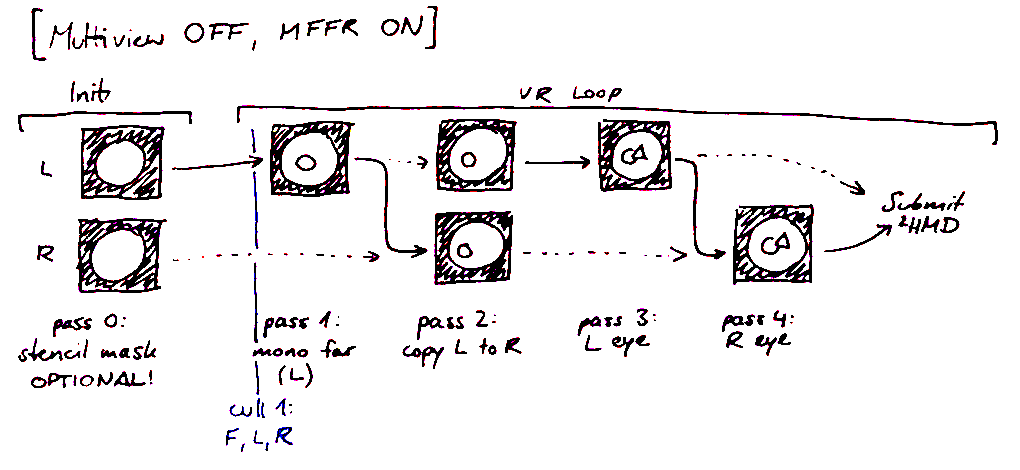
\includegraphics[width=0.9\textwidth]{pictures/flowchart_mffr}
  \caption{[TODO: Monoscopic Far-Field rendering flowchart]} \label{fig:flowchart_mffr}
\end{figure}

\subsection{Estimated impact}
The makeup of the scene itself will also affect effectiveness of the solution. As cautioned by Oculus LLC in their developer reference on Mono Far-Field Rendering [TODO: src], there is a certain baseline overhead simply for enabling the additional render pass necessary for the monoscopic image and the associated context switches. Furthermore only scenes with a significant of distant geometry beyond the field split distance will benefit from the optimization, as obviously the second view workload can only be saved for objects that would be contained within that second pass. 
[TODO]

\subsection{Implementation specifics}
[TODO]



\section{MFFR Variant: Depth Shift}
[TODO]

\section{MFFR Variant: Alternate eye}
[TODO]
